So far we have not made any assumptions regarding the cause of variability of the source term, \ie, the power term, in the thermal system given by \eref{fourier-system}.
In this section, a particular application of the proposed framework.
Specifically, we shall perform stochastic PTA of a multiprocessor platform wherein the uncertainty originates from the leakage power via the variability of the effective channel length due to process variation.
The effective channel length has one of the strongest effects on the leakage current and, consequently, on power and temperature \cite{juan2011, juan2012}; at the same time, this crucial parameter is severely deteriorated by process variation \cite{chandrakasan2001, srivastava2010}.

\subsection{Problem Formulation} \slabel{ie-problem-formulation}
The total dissipation of power is composed of two major parts: dynamic and static.
The influence of process variation on the dynamic power is known to be negligibly small \cite{srivastava2010}; on the other hand, the variability of the static power is substantial, in which the subthreshold leakage current contributes the most \cite{juan2011, juan2012}.
Hence, we shall focus on the subthreshold leakage and, more specifically, on the effective channel length, denoted by $\Leff$, since it has the strongest influence on leakage and is severely deteriorated by process variation \cite{chandrakasan2001}.
In particular, $\Leff$ also affects the threshold voltage \cite{juan2011}.

It is well known that the dispersion due to process variation of the effective channel length around the nominal value resembles a bell shape, which is similar to the ones owned by Gaussian distributions.
Therefore, such variations are often conveniently modeled using Gaussian variables \cite{srivastava2010, juan2011, juan2012, chandra2010, huang2009, lee2013, shen2009, bhardwaj2006, ghanta2006}.
In this work, due to both the underlying physics and demonstration purposes, we make a step further and bake right into the model the fact that the effective channel length---occupying the space between the drain and source of a nanoscopic transistor---cannot be arbitrarily large or take a negative value, as Gaussian distributions allow it to do.
In other words, we require the model of $\Leff$ to have a bounded support.
With this in mind, we propose to model physically-bounded parameters using the four-parametric family of beta distributions: $\dBeta(a, b, c, d)$ where $a$ and $b$ are the shape parameters, and $c$ and $d$ are the left and right bounds of the support, respectively.
$a$ and $b$ can be chosen in such a way that the typically found bell shape of the distribution is preserved.
An illustration is given in \fref{beta-normal} where we fitted a beta distribution to the standard Gaussian distribution.\footnote{Alternatively, one can match the moments of the distributions.}
It can be seen that the curves are nearly indistinguishable, but the beta one has a bounded support $[-4, 4]$, which can potentially lead to more realistic models.

\begin{figure}[t]
  \centering
  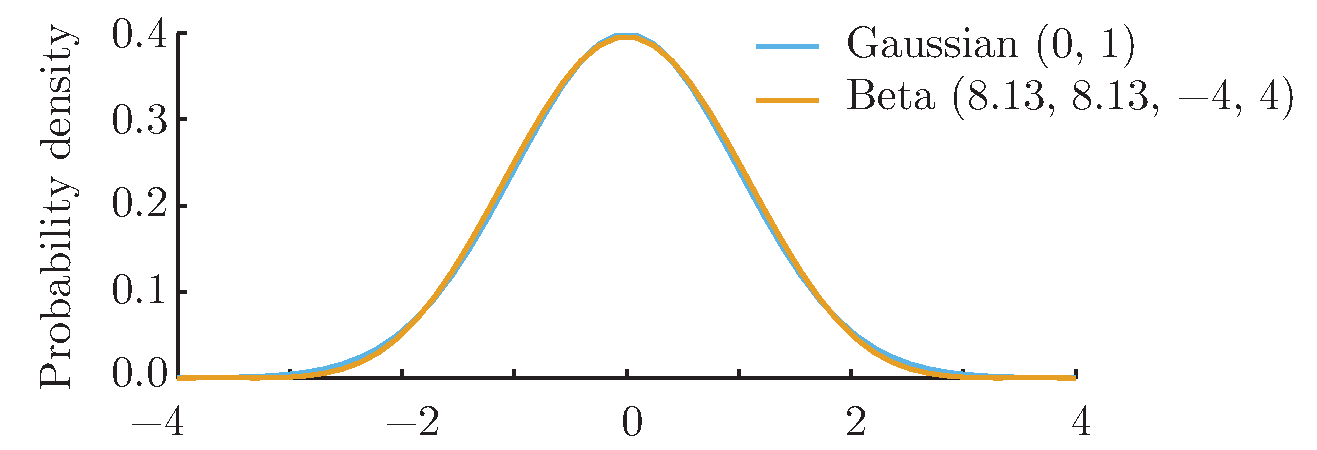
\includegraphics[width=0.9\ColumnWidth]{include/assets/beta-normal.pdf}
  \caption{The standard Gaussian distribution and a fitted beta distribution.}
  \flabel{beta-normal}
\end{figure}

The variability of $\Leff$ is split into global $\gLeff$ and local $\lLeff$ parts \cite{chandra2010, shen2009}.\footnote{Without loss of generality, $\gLeff$ can be treated as a composition of independent inter-lot, inter-wafer, and inter-die variations; likewise, $\lLeff$ can be treated as a composition of independent and dependent local variations.}
$\gLeff$ is assumed to be shared among all processing elements whereas each processing element has its own local parameter $\lLeff_i$.
Therefore, the effective channel length the $i$th processing element is modeled as follows:
\begin{equation} \elabel{leakage-partition}
  \Leff_i = \nLeff + \gLeff + \lLeff_i
\end{equation}
where $\nLeff$ is the nominal value of the effective channel length.
Hence, the uncertain parameters of the problem are
\begin{equation} \elabel{uncertain-parameters}
  \vU = \vec{\lLeff_1, \dotsc, \lLeff_\nprocs, \gLeff}.
\end{equation}

Global variations are typically assumed to be uncorrelated with respect to the local ones.
The latter, however, are known to have high spatial correlations, which we shall model using the following correlation function:
\begin{equation} \elabel{correlation-function}
  \fCorr(\vR_i, \vR_j) = \eta \; \fCorrSE(\vR_i, \vR_j) + (1 - \eta) \fCorrOU(\vR_i, \vR_j)
\end{equation}
where $\vR_i \in \real^2$ is the spatial location of the center of the $i$th processing element relative to the center of the die. The correlation function is a composition of two kernels:
\begin{align*}
  & \fCorrSE(\vR_i, \vR_j) = \exp\left(- \frac{\norm{\vR_i - \vR_j}^2}{\lCorrSE^2} \right) \text{ and} \\
  & \fCorrOU(\vR_i, \vR_j) = \exp\left(- \frac{\abs{\,\norm{\vR_i} - \norm{\vR_j}\,}}{\lCorrOU} \right),
\end{align*}
which are known as the squared-exponential and Ornstein-Uhlenbeck kernels, respectively.
$\eta \in [0, 1]$ is a weight coefficient balancing the kernels; $\lCorrSE$ and $\lCorrOU > 0$ are so-called length-scale parameters; and $\norm{\cdot}$ stands for the Euclidean distance.
The choice of the correlation function in \eref{correlation-function} is guided by the observations of the correlations induced by the fabrication process \cite{chandrakasan2001, friedberg2005, cheng2011}: $\fCorrSE$ imposes similarities between the spatial locations that are close to each other, and $\fCorrOU$ imposes similarities between the locations that are at the same distance from the center of the die (see also \cite{huang2009, ghanem1991, lee2013, bhardwaj2008, ghanta2006}).
The length-scale parameters $\lCorrSE$ and $\lCorrOU$ control the extend of these similarities, \ie, the range wherein the influence of one point on another is significant.

Although \eref{correlation-function} captures certain features inherent to the fabrication process, it is still an idealization.
In practice, it can be difficult to make a justifiable choice and tune such a formula, which is a prerequisite for the techniques in \sref{prior-work} based on the (continuous) KL decomposition.
A correlation matrix, on the other hand, can readily be estimated from measurements and, thus, is a more probable input to PTA.
Thus, we use \eref{correlation-function} with the only purpose of constructing a correlation matrix of $\{ \lLeff_i \}$.
For convenience, the resulting matrix is extended by one dimension to pack $\gLeff$ and $\{ \lLeff_i \}$ together.
In this case, the correlation matrix obtains one additional non-zero element on the diagonal.
Taking into account the variances of the variable, the final covariance matrix of the whole random vector $\vU$ (see \eref{uncertain-parameters}) is formed, which we denote by $\mCov_\vU$.

To conclude, an input to our analysis is the marginal distributions of the parameters $\vU$, which are beta distributions, and the corresponding covariance matrix $\mCov_\vU$.


\subsection{Uncertain Parameters} \slabel{ie-uncertain-parameters}
The total dissipation of power is composed of two major parts: dynamic and leakage. The influence of process variation on the dynamic power is known to be negligibly small \cite{juan2011, juan2012, srivastava2010}; on the other hand, the variability of leakage is substantial, wherein the subthreshold current contributes the most \cite{juan2011, juan2012}. Hence, we focus on the subthreshold leakage and, more specifically, on the effective channel length denoted by $\Leff$. The variations of $\Leff$ are split into global (inter-die) and local (intra-die) parts \cite{chandra2010, juan2011, juan2012, srivastava2010, shen2009}. The global contribution is shared among all the processing elements and, therefore, is modeled as a single \rv\ $\gLeff(\o)$; furthermore, $\gLeff(\o)$ is typically assumed to be independent with respect to the local variations. The latter, however, are known to have high spatial correlations, which, due to particularities of the manufacturing process, often bear radial structures \cite{friedberg2005, cheng2011}. Therefore, as in \cite{ghanta2006}, we model the intra-die variations as a continuous-space stochastic process $\lLeff(r, \o)$ with the following radial covariance function \cite{ghanem1991}:
\begin{equation} \elabel{covariance-function}
  \fCov{\lLeff}{r_i, r_j} = e^{-|r_i - r_j|/\corrLength}
\end{equation}
where $r_i$ is the distance from the $i$th processing element to the center of the die, and $\corrLength$ is the correlation length. In words, the structure implies that the smaller the radial distance between two processing elements on the die, the more likely they are to have similar deviations of the effective channel length. Finally, it is generally accepted that the variations of the channel length have Gaussian distributions \cite{juan2011, juan2012, srivastava2010}. Therefore, we assume that the \rv\ $\gLeff(\o)$ as well as the process $\lLeff(r, \o)$ are Gaussian.

$\gLeff(\o)$ and $\lLeff(r, \o)$ form the input set of uncertain parameters $\vU(r, \o)$, which is to be processed in order to extract a finite set of mutually independent \rvs\ $\vZ(\o)$. Following the guidelines in \sref{uncertain-parameters}, Stage~1, the KL expansion suits the best in such a situation. A thorough elaboration on KL is out of the scope of this paper; however, the interested reader is referred to \aref{uncertain-parameters} where KL is applied to \eref{covariance-function}.


\subsection{Power and Thermal Models} \slabel{ie-power-model} \slabel{ie-thermal-model}
The (total) power dissipation of the system with $\cores$ processing elements is given as the following sum:
\begin{equation} \elabel{power-model}
  \vP(\t, \o) = f_\dyn(\vP_\dyn(\t), \o) + f_\leak(\vTO(\t, \o), \o)
\end{equation}
where $f_\dyn, f_\leak: \real^\cores \times \outcomes \to \real^\cores$ model the dynamic and leakage power, respectively, as functions of the uncertain parameters $\vZ(\o)$. In addition, $f_\dyn$ depends on the nominal dynamic power $\vP_\dyn \in \real^\cores$, and the leakage part, $f_\leak$, depends on the operating temperature $\vTO \in \real^\cores$ due to the well-known non-linear interdependency between leakage and temperature, c.f. \cite{srivastava2010, liu2007}. We do not impose any further restrictions on $f_\dyn$ and $f_\leak$, and let the user to decide\footnote{One can easily find a dicent number of alternatives in the contemporary literature, for instance, follow the reference in \cite{srivastava2010}.}. Moreover, the functions are not required to have explicit mathematical formulations; they can be given as a `black box' as long as its inputs are in the set $\{ \vP_\dyn, \vTO, \vZ \}$.


\subsection{Surrogate Model} \slabel{ie-polynomial-chaos}
At \stage{4}, the independent \rvs, power model, and thermal model are fused together under the desired workload, $\profilePdyn$, to produce the corresponding stochastic power $\profileP{\o}$ and temperature $\profileT{\o}$ profiles. The obtained stochastic profiles are nothing more than two polynomials of $\Z_1(\o)$ and $\Z_2(\o)$ with time-dependent coefficients.

The construction of PC expansions is based on the Hermite basis (see \tref{askey}) as it was found to be optimal in situations involving Gaussian parameters \cite{xiu2010}.
A one-dimensional example of the basis is given in \fref{hermite} where the first six Hermite polynomials $\{ \pcb_i(\z) \}_{i = 1}^6$ are displayed.

In two dimensions, assuming a second-total-order PC expansion, the temperature at the $k$th moment of time is
\begin{align*}
  \vTO_k(\o) &= \pccs_{k1} + \pccs_{k2} \Z_1(\o) + \pccs_{k3} \Z_2(\o) + \pccs_{k4} \Z_1(\o) \Z_2(\o) \\
  & \qquad \qquad {} + \pccs_{k5} (\Z_1(\o)^2 - 1) + \pccs_{k6} (\Z_2(\o)^2 - 1)
\end{align*}
where $\pccs_{ki}$ are vectors with two elements corresponding to the two processors.

Once the basis has been chosen, we need to compute the corresponding coefficients, specifically, $\pcc{\vP}_i$ in \eref{pc-expansion}. As shown in \aref{polynomial-chaos}, the computation of $\pcc{\vP}_i$ involves multidimensional integration with respect to the \pdf\ of the \rvs\ $\vZ(\o)$.
In numerical analysis, this task is typically accomplished by virtue of a quadrature rule \cite{press2007}, which, loosely speaking, is a weighted summation over the integrand values computed at prescribed points. A natural choice of a quadrature rule when the weight function is a Gaussian \pdf\ is the Gauss-Hermite quadrature. Further details are given in \aref{gauss-quadrature}.

To summarize, we have completed four out of five stages of the proposed UQ framework depicted in \fref{algorithm}. The result is a light surrogate of the model in \eref{fourier-system}. At each moment of time, the surrogate is composed of two $\nprocs$-valued polynomials, one for power and one for temperature, that are defined in terms of $\nvars$ mutually independent \rvs; an example of such a polynomial is given in \eref{pc-k}. The constructed representation can be trivially analyzed to retrieve various statistics of the system in \eref{fourier-system}, and this is \stage{5}\ in \fref{algorithm}, which will be illustrated as a part of the next section.

\begin{figure}
  \centering
  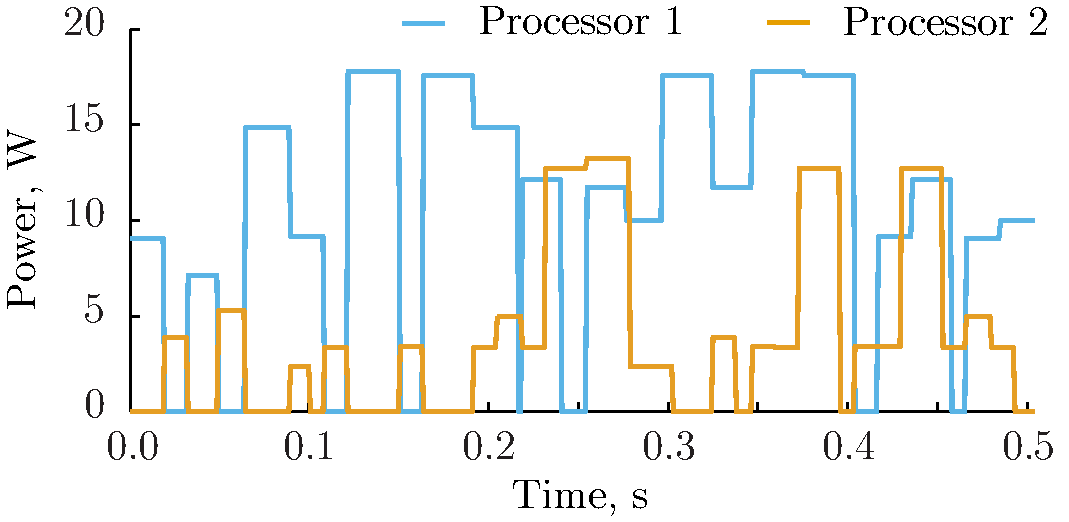
\includegraphics[width=1.00\columnwidth]{include/assets/application-power.pdf}
  \vspace{-0.5em}
  \caption{A dynamic power profile.}
  \flabel{application-power}
  \vspace{-0.5em}
\end{figure}

Assume that the dynamic power profile, $\profilePdyn$, corresponding to the considered workload is the one shown in \fref{application-power}.

\begin{figure}[bl]
  \vspace{-1.0em}
  \centering
  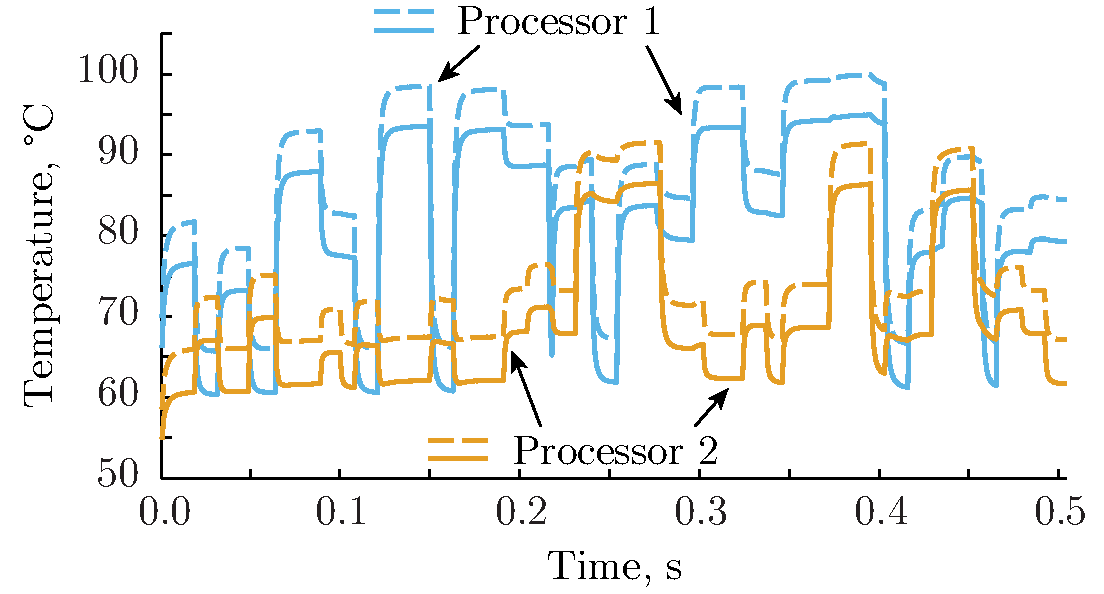
\includegraphics[width=0.90\columnwidth]{include/assets/application-temperature.pdf}
  \vspace{-0.5em}
  \caption{The expected temperature (the solid lines) and one standard deviation above it (the dashed lines).}
  \flabel{application-temperature}
\end{figure}

The expansion for power has the same structure but different coefficients.
Such a series might be shorter or longer depending on the accuracy requirements.
As we see, our surrogate model has a negligibly small computational cost to undertake UQ at \stage{5}: for any outcome of the uncertain parameters $\vZ(\o) \equiv \vZ$, we can easily compute the corresponding temperature by plugging $\vZ$ into the above equation; the same applies for power.
Thus, such characteristics as \cdfs\ and \pdfs\ (see \fref{motivation-pdf}) can be rigorously estimated. Furthermore, the expectation and variance at the $k$th moment of time are calculated as simply as
\[
  \oExp{\vTO_k(\o)} = \pccs_{k1} \hspace{1em} \text{and} \hspace{1em} \oVar{\vTO_k(\o)} = \sum_{i = 2}^{6} \pcn_i \: \pccs_{ki}^2
\]
where $\pcn_i$ are normalization constants, and the squaring should be understood element-wise.
For the nominal power profile $\profilePdyn$ depicted in \fref{application-power}, we obtain the corresponding stochastic temperature profile $\profileT{\o}$ and can observe, \eg, its expectation and standard deviation; they are plotted in \fref{application-temperature}.
The displayed curves closely match those obtained via MC simulations with $10^4$ samples; however, our method takes less than a second, on a personal laptop, while MC sampling takes more than a day, which we discuss in \sref{experimental-results}.

